\documentclass[conference]{IEEEtran}
\IEEEoverridecommandlockouts
% The preceding line is only needed to identify funding in the first footnote. If that is unneeded, please comment it out.
\usepackage{cite}
\usepackage{amsmath,amssymb,amsfonts}
\usepackage{algorithmic}
\usepackage{graphicx}
\usepackage{textcomp}
\usepackage{xcolor}
\def\BibTeX{{\rm B\kern-.05em{\sc i\kern-.025em b}\kern-.08em
    T\kern-.1667em\lower.7ex\hbox{E}\kern-.125emX}}
\begin{document}

\title{PAE Gruppe 1*\\
{\footnotesize \textsuperscript{*}Note: Sub-titles are not captured in Xplore and
should not be used}
\thanks{Identify applicable funding agency here. If none, delete this.}
}

\author{\IEEEauthorblockN{1\textsuperscript{st} Given Name Surname}
\IEEEauthorblockA{\textit{dept. name of organization (of Aff.)} \\
\textit{name of organization (of Aff.)}\\
City, Country \\
email address or ORCID}
\and
\IEEEauthorblockN{2\textsuperscript{nd} Given Name Surname}
\IEEEauthorblockA{\textit{dept. name of organization (of Aff.)} \\
\textit{name of organization (of Aff.)}\\
City, Country \\
email address or ORCID}
\and
\IEEEauthorblockN{3\textsuperscript{rd} Given Name Surname}
\IEEEauthorblockA{\textit{dept. name of organization (of Aff.)} \\
\textit{name of organization (of Aff.)}\\
City, Country \\
email address or ORCID}
\and
\IEEEauthorblockN{4\textsuperscript{th} Given Name Surname}
\IEEEauthorblockA{\textit{dept. name of organization (of Aff.)} \\
\textit{name of organization (of Aff.)}\\
City, Country \\
email address or ORCID}
}

\maketitle

\begin{abstract}

\end{abstract}

\section{Use Case (JG)}

\begin{figure}[htbp]
	\centering
	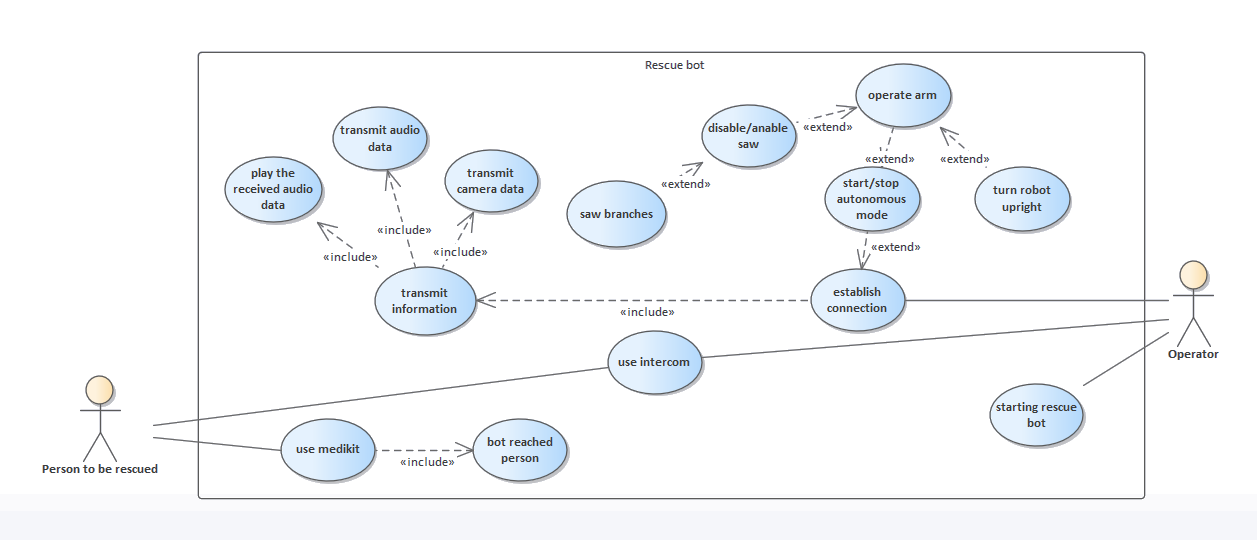
\includegraphics[width=0.5\textwidth]{Use-Case}
	\caption{Use Case}
\end{figure}

Nach der Erstellung der Anforderungen haben wir ein Use Case Diagramm erstellt.\newline 
In Fig. 1 ist das Use Case Diagramm zusehen. Außerhalb stehen die Aktoren "Operator" und "Person to be rescued", als Strichmännchen dargestellt. Innerhalb sind die Funktionen des rescue bots dargestellt und wie diese mit den Aktoren verbunden sind. Die Use Cases sind mit inludes oder extends untereinander verbunden. Die Aktoren sind durch Assoziationen mit den Use Cases verbunden. Zum Beispiel kann der Operator den rescue bot starten. Dann stellt der Operator eine Verbindung mit dem rescue bot her. Über die Verbindung zum rescue bot werden verschiedene Informationen, wie Kamera Daten und Audio Daten übermittelt. Der Operator kann zwischen Autonomen und manuellen Modus wechseln. Im manuellen Modus kann der Operator den Arm bedienen. Zudem kann er eine Säge aktivieren oder deaktivieren um Äste zu durchsägen.
Der Arm kann auch dafür benutzt werden, den rescue bot wieder aufzustellen wenn er auf die Seite gefallen ist.
Wenn der rescue bot die zu rettende Person erreicht hat, kann der Operator über eine Gegensprechanlage die Person ansprechen. Zum schluss kann die zu rettende Person ein medikit benutzen, um selbst kleine Verletzungen zu versorgen.




\section{Stakeholder (JG)}
Um mögliche Risiken oder Blockaden, die das Projekt stoppen oder zum Abbruch bringen können zu finden haben wir eine Stakeholderanalyse durchgeführt. Stakeholder sind alle Personen, die mit dem Projekt in Kontakt kommen. Dazu gehören z.B. der Arbeitgeber, das Rettungsteam, die zu rettende Person (Opfer), Finanzmanager und der TÜV.
\\


\subsection{Rettungshelfer}
Die Rettungshelfer wollen sich selbst und dritte nicht zusätzlich in gefährlichen Situationen in Gefahr bringen.
Die Lösung dafür ist, das der Roboter anwendbar für Situationen die zu Gefährlich für die Rettungshelfer sind gemacht wird.

\subsection{Menschen die gerettet werden}

Die zu rettenden Menschen wollen eine schnelle medizinische Hilfe und schnelle Rettung.
Hier ist die Lösung, das der zu rettende Mensch so schnell und sanft wie möglich gerettet wird.

\subsection{Familie des zu rettenden Menschen}

Die Familie des zu rettenden Menschen will wissen, das ihre Verwandtschaft in Sicherheit ist.
Um der Familie dies zu bieten, muss dem zu rettenden Menschen die best mögliche Rettung geliefert werden.

\subsection{Finanzmanager}

Der Finazminister will ein Produkt mit einem hohen Mehrwert zu möglichst niedrigen kosten.
Dazu ist die Lösung, ein System mit einem guten Preis-Leistungsverhältnis zu entwickeln.

\subsection{Arbeitgeber}

Der Arbeitgeber möchte ein verkaufbares Prokdut mit einer hohen verkaufsrate und einem hohen Profit.
Die Lösung ist, eine System mit hoher Sicherheit aufzubauen, um eine Entschädigung zu vermeiden und einen Kaufanreiz zu schaffen, der auch mit einem hohen Profit möglich ist.

\subsection{TÜV}

Der TÜV möchte Sicherheit für alle Beteiligten, wie Rettungshelfer, Menschen die gerettet werden sollen und Dritte.
Um dies einzuhalten müssen Richtlinien eingehalten und ein sicheres System eingerichtet werden, um eine TÜV-Zertifizierung zu bekommen. 

\subsection{Kunden}

Der Kunde will, das die Rettungshelfer gut ausgestattet sind.
Dazu wird der rescue bot(Ausstattung) in regelmäßigen abständen gewartet. Zudem gibt es eine Kundenbetreuungen um sie mit dem neuen Produkt vertraut zu machen. Dies ist wichtig um mögliche bedenken zu dem rescue bot beiseite zu schaffen.
\\

\subsection{Stakeholder matrix}

\begin{figure}[htbp]
	\centering
	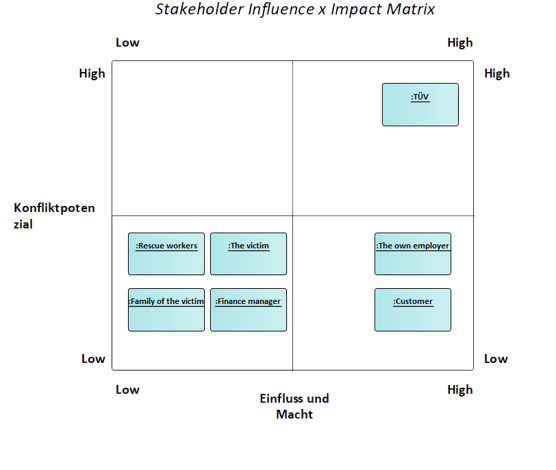
\includegraphics[width=0.5\textwidth]{Stakeholder-Matrix}
	\caption{Stakeholder-Matrix}
\end{figure}

In Fig. 2 ist die Stakeholder-Matrix mit den verschiedenen Stakeholdern zusehen. Die Stakeholder haben wir nach "Einfluss und Macht" und Konfliktpotential sortiert. Die Rettungshelfer, die zu rettende Person, die Familie der zu rettenden Person und der Finanzmanager haben am wenigsten Einfluss und Macht und am wenigsten Konfliktpotenzial in dem Projekt. Diese Stakeholder können kaum bis gar nichts in dem Projekt mit entscheiden. Zum Beispiel will der Finanzmanager ein Produkt mit einem guten Preis-Leistungsverhältnis wie in Kapitel D beschrieben. Was das Projekt am Ende kostet kann der Finanzmanager jedoch nicht beeinflussen. Viel Einfluss aber wenig Konfliktpotential hat der Arbeitgeber und der Kunde. Zum Beispiel kann der Arbeitgeber viel mit entscheiden, was gemacht werden kann und was nicht. Zudem hat der Kunde eine Vorstellung von dem was er will und kann so starken Einfluss auf das Projekt haben. Der TÜV hat ein hohes Konfliktpotenzial und viel Einfluss und Macht. Durch z.B. fehlenden Sicherheitsmaßnahmen kann der TÜV das Projekt zum Abbruch bringen. 


\section{Activity Diagramm (JG)}

Nachdem das Use Case Diagramm erstellt wurde, haben wir ein Aktivitätsdiagramm bezüglich des autonomen Fahrens, wie in Fig. 3 gezeigt, erstellt. Die erste Aktivität ist, das der Operator sich mit dem Rescue bot über das Remotecontroll und dem remote verbindet. Weiter geht es mit der Sensorauslesung und der Evaluierung der Sensordaten. Darüber überprüft er auf Wasser und entscheidet sich bei "water" für über Wasser fahren und bei "no water" für über Land fahren. Die nächste Aktivität ist, das auf Audiosignale überprüft wird. Bei erkanntem Signal folgt der rescue bot dem Signal, ansonsten fährt er gerade aus weiter. Parallel dazu wird die camera über das remote controll aktiviert. Dazu gehören die Aktivitäten send data, receive data und display video. Wenn ein object erkannt wird, wird das Objekt Identifiziert. Ein Objekt wird unterschieden zwischen nicht identifizierbar, identifiziert als sägbares Objekt und identifiziert als Person. Bei einem zersägbaren Objekt wird nachgefragt ob der rescue bot im Autonomen modus ist. Ist der bot nicht im autonomen Modus, wird der bot gestoppt und der remotecontroll (arm/säge) kann verwendet werden. Danach wird abgefragt ob der bot wartet. Wenn ja, dann wird dem rescue bot erlaubt weiter zu fahren. Sollte das Objekt nicht identifizierbar sein, wird es einfach umfahren. Wurde die Person identifiziert, wird abgefragt ob die Person erreicht wurde. Über jeden weg wird abgefragt, ob die Person erreicht wurde. Also nach der Hindernisumfahrung, dem Äste zersägen. Wurde die Person nicht erreicht, werden die Sensoren wieder ausgelesen und so weiter. Wenn sie erreicht wurde, stoppt der rescue bot und der Operator kann mit der Person reden. Zum Schluss fährt der rescue bot zurück.

\begin{figure}[htbp]
	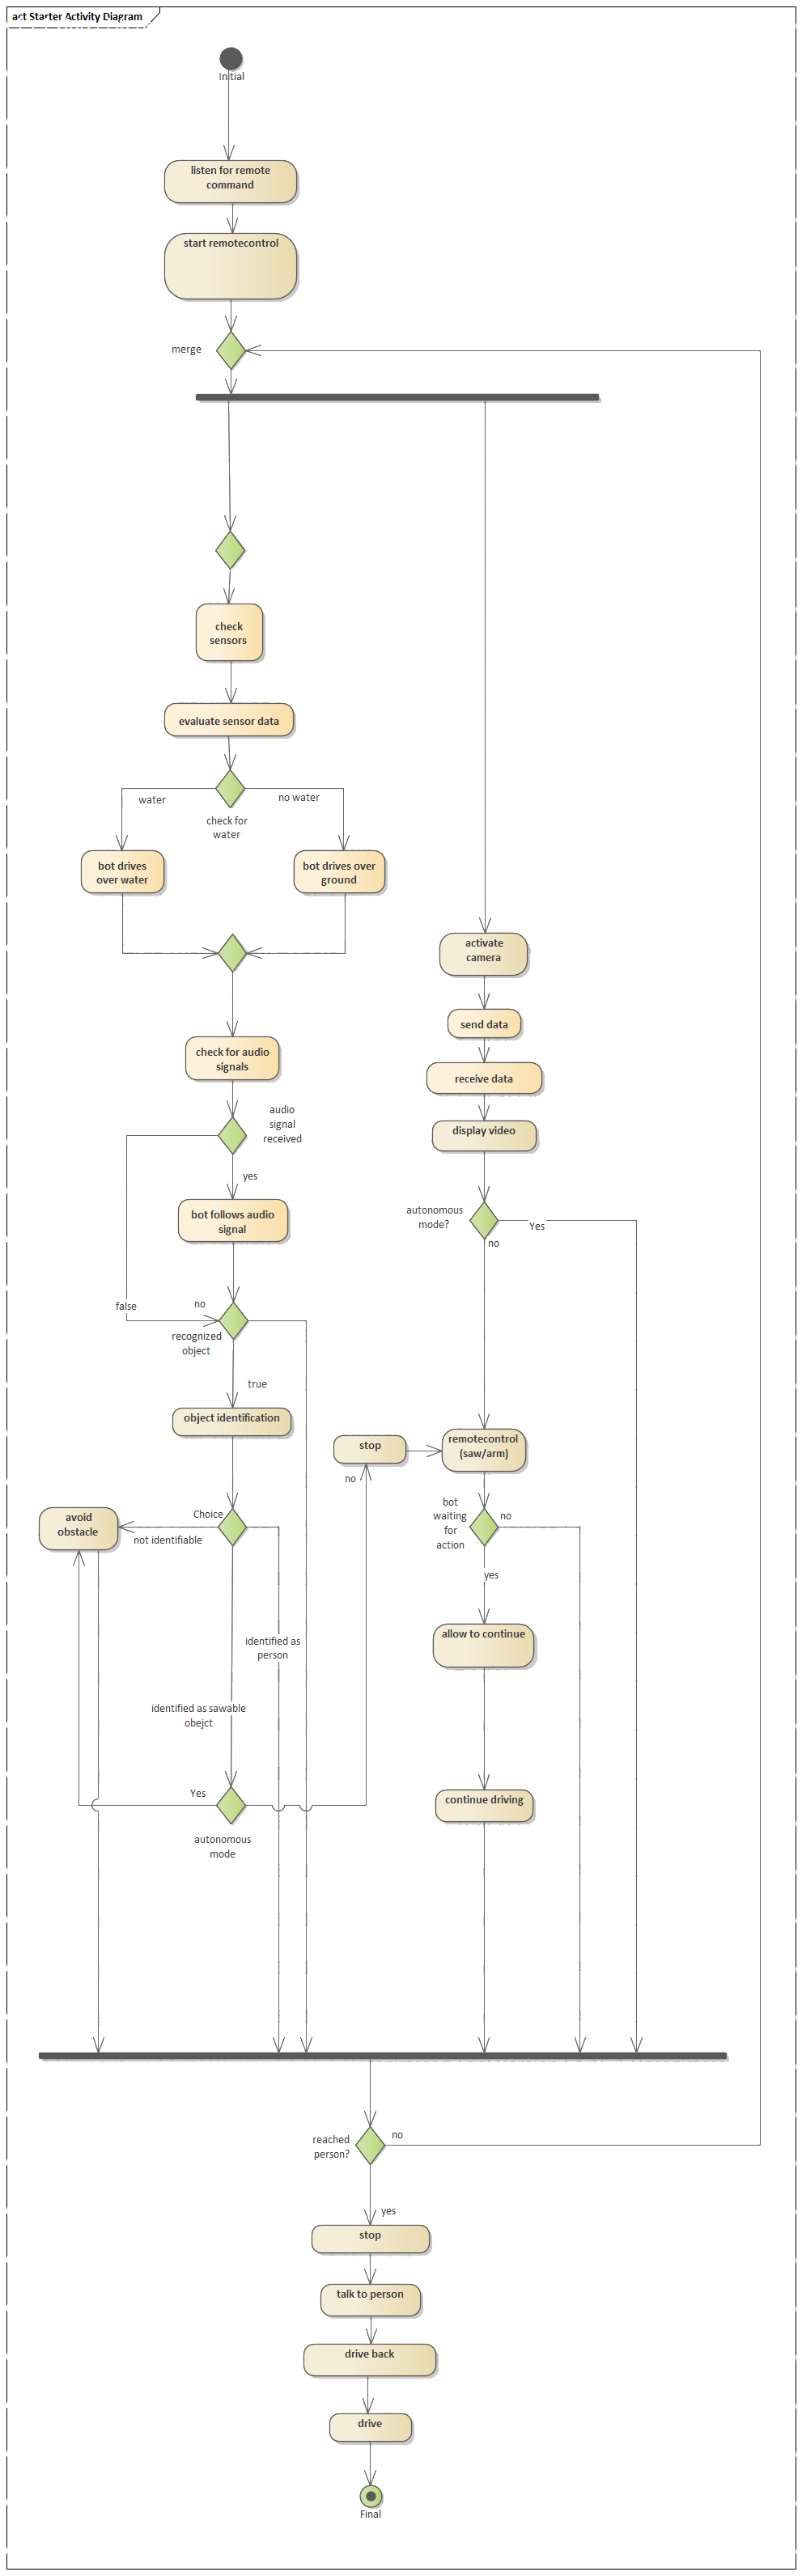
\includegraphics[width=0.4\textwidth]{Activity Diagram}
	\caption{}
	\label{fig:Bild1}
\end{figure}

\newpage

\section{Swimlane (JG)}

In Fig. 4 ist das "Swimlane diagramm" zusehen. Hier wurden die verschiedenen Aktivitäten aus dem Aktivitätsdiagramms nach Sensorcontroller (Blau), Hauptcontroller (Gelb), Motorcontroller (Lila), Objekterkennung (Grün), Remotecontrol (Orange) und remote (Rot) Kategorisiert. Es ist notwendig den rescue bot mit dem remote zu verbinden. Erst danach kann der rescue bot losfahren und die Sensoren auslesen.
Der Sensorcontroller ließt die Sensoren aus und der Hauptcontroller evaluiert sie. Über diese Informationen wird der Motorcontroller angesteuert, ob er auf Land oder Wasser fahren soll. Weiter gibt der Hauptcontroller über empfangene Audiosignale den Befehl, das der rescue bot dem Signal folgen soll. In der Kategorie Objekterkennung unter Objekt Identifizierung wird zwischen nicht identifizierbar, identifiziert als sägbares Objekt und identifiziert als Person unterschieden. Bei einem als zersägbares Objekt identifiziertes Objekt, werden über den Motorcontroller die Motoren gestoppt und der Operator kann über das remote die äste durchsägen. Danach erlaubt der Operator dem rescue bot über die remotesteuerung das weiterfahren. Nachdem die zu rettende Person erreicht wurde, bekommt der Motorcontroller das Signal, die Motoren anzuhalten. Der Operator kann nun über das remote und der Gegensprechanlage mit der zu rettenden Person reden. Am Ende fährt der rescue bot zurück zum Startpunkt.  

\begin{figure}[htbp]
	\centering
	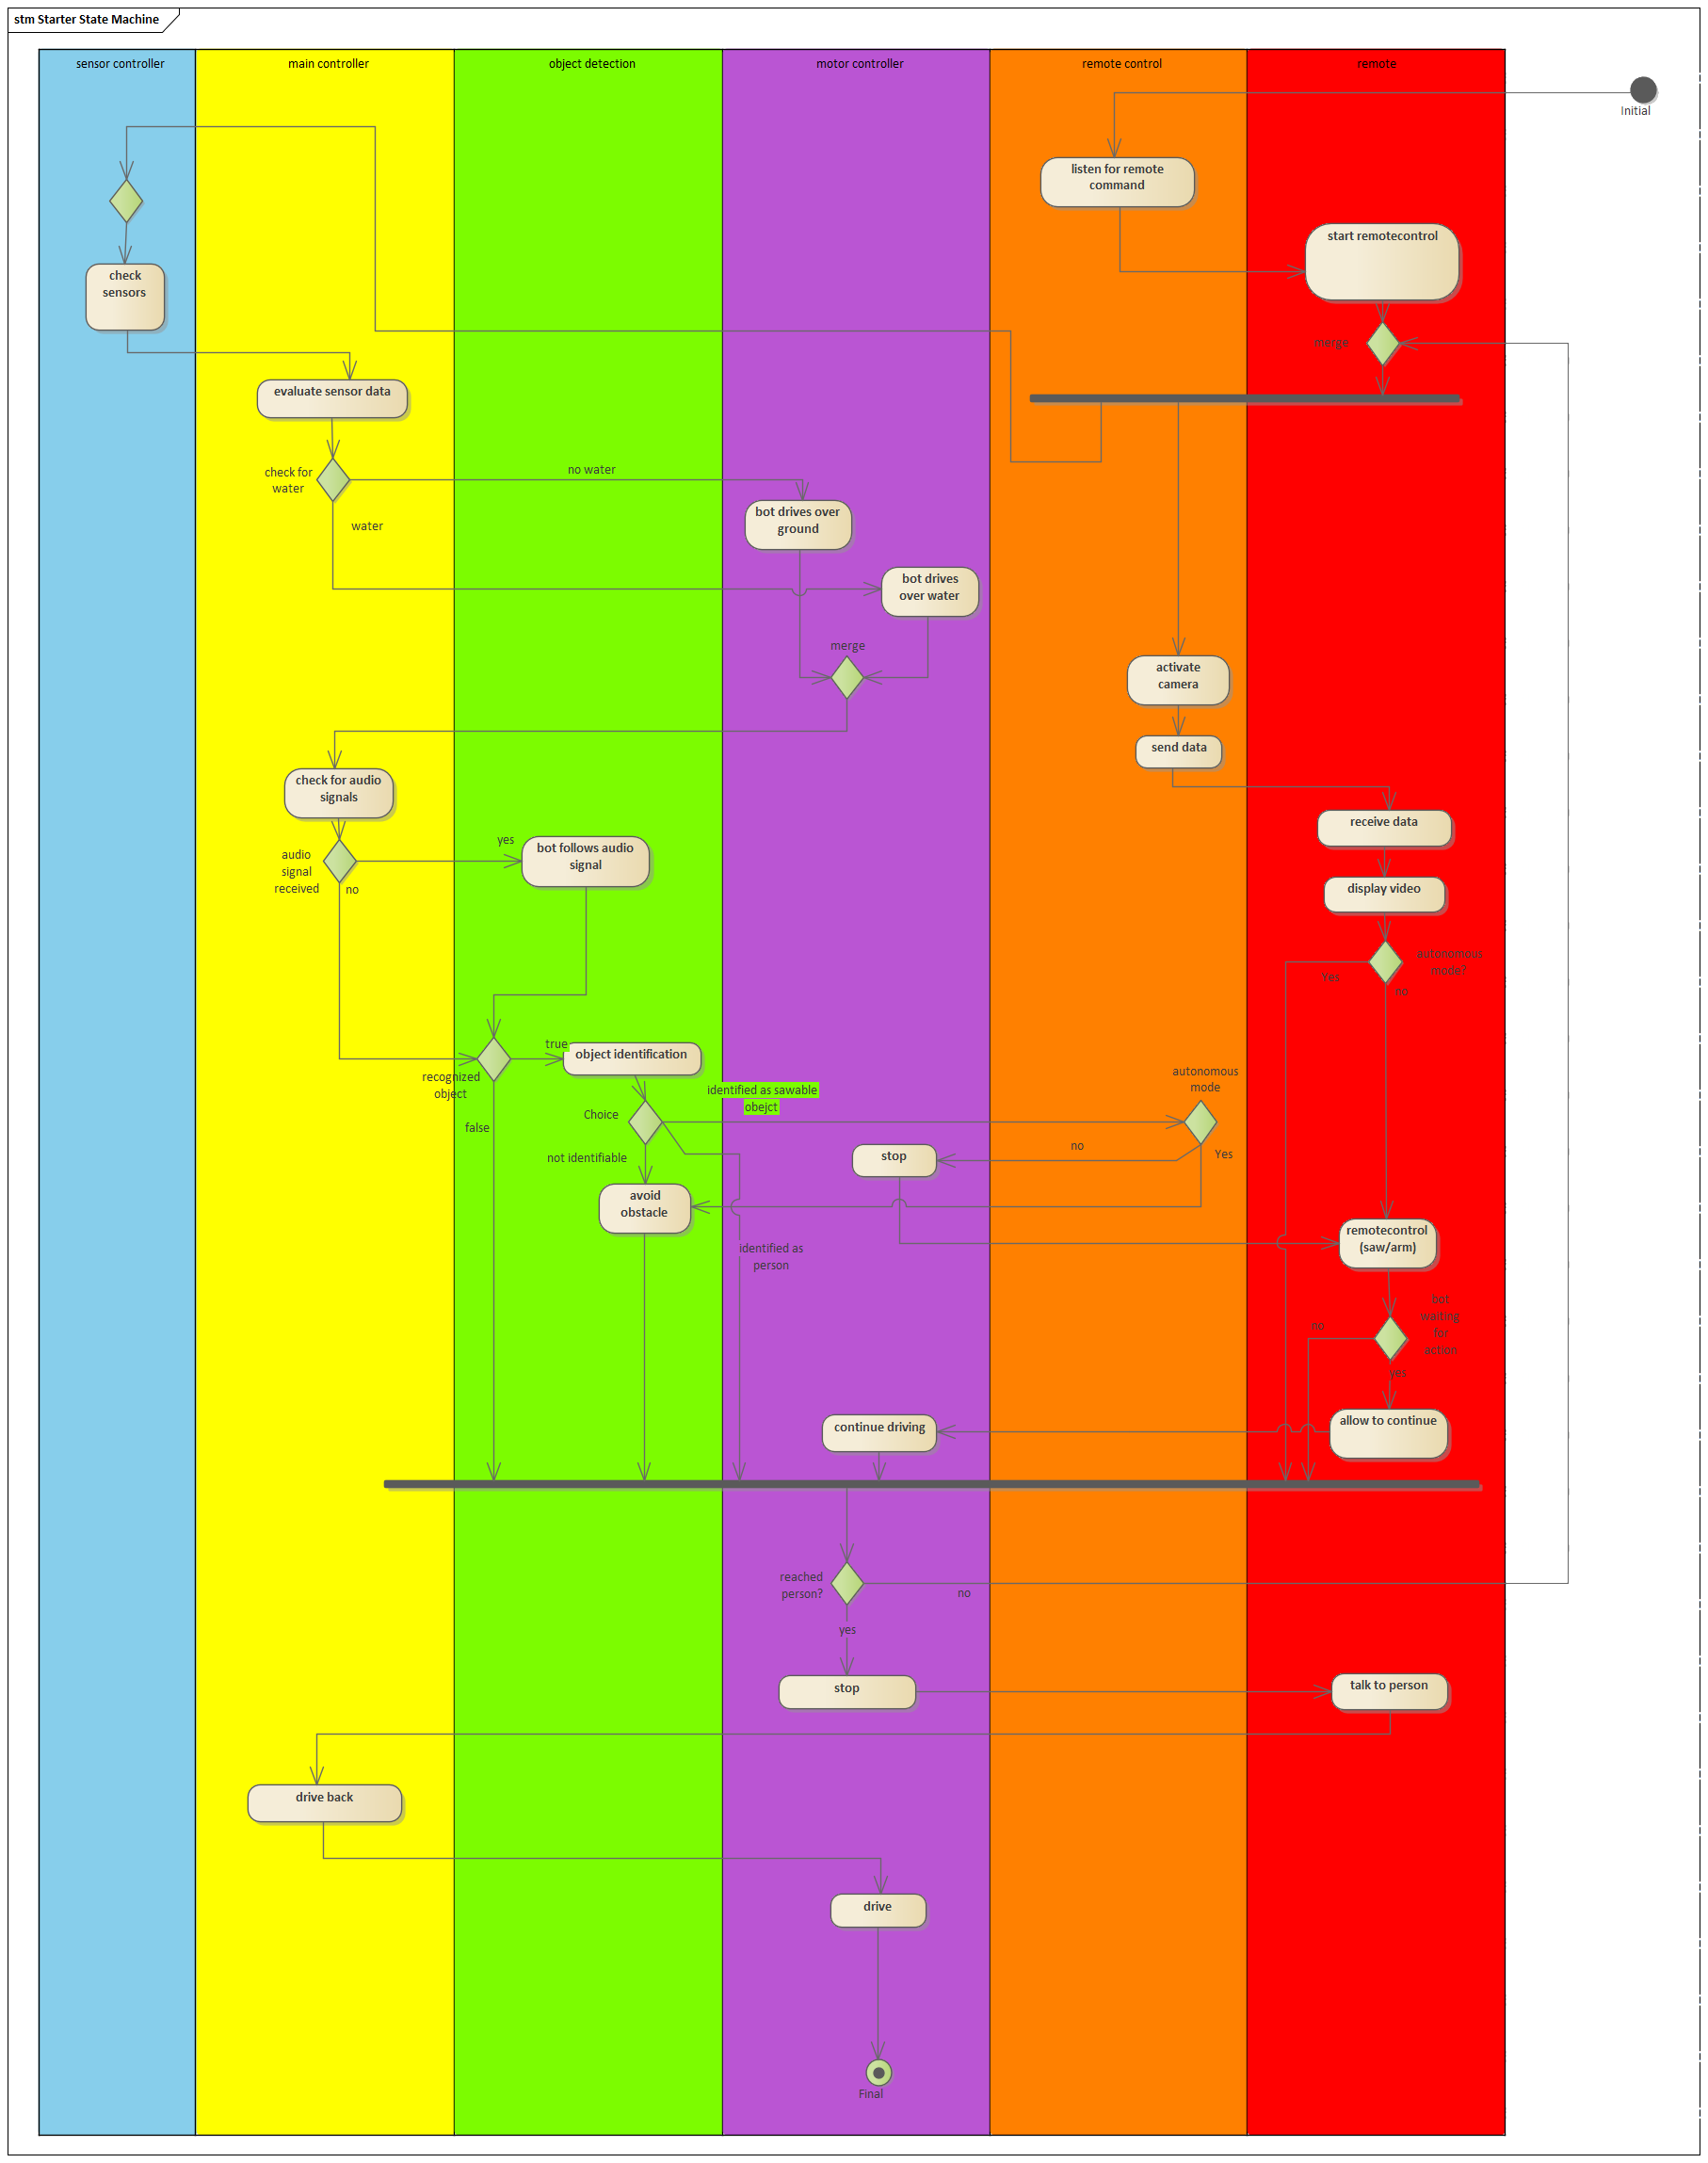
\includegraphics[width=0.5\textwidth]{Starter State Machine1}
	\caption{Swimlane}
	
\end{figure}



\section*{References}



\vspace{12pt}
\color{red}


\end{document}
